\documentclass[pdf]{beamer}

\usetheme{Warsaw}

\usepackage{alltt}

\usepackage{amssymb, amsmath}

\usepackage[english]{babel}

\usepackage{tikz}
\usetikzlibrary{calc,trees,positioning,arrows,chains,automata,shapes.geometric,%
    decorations.pathreplacing,decorations.pathmorphing,shapes,%
    matrix,shapes.symbols}

\usetikzlibrary{shapes,arrows,automata,positioning,calc}
\usetikzlibrary{fit,backgrounds}
\usetikzlibrary{decorations.pathreplacing}
\tikzset{
>=stealth',
  punktchain/.style={
    rectangle,
    rounded corners,
    % fill=black!10,
    draw=black, very thick,
    text width=6em,
    minimum height=3em,
    text centered,
    on chain},
  line/.style={draw, thick, <-},
  element/.style={
    tape,
    top color=white,
    bottom color=blue!50!black!60!,
    minimum width=8em,
    draw=blue!40!black!90, very thick,
    text width=10em,
    minimum height=3.5em,
    text centered,
    on chain},
  every join/.style={->, thick,shorten >=1pt},
  decoration={brace},
  tuborg/.style={decorate},
  tubnode/.style={midway, right=2pt},
}

% collection of macros used in the paper

%Learners
\newcommand{\learnlib}{LearnLib}

\newcommand{\A}{{\mathcal A}}
\newcommand{\B}{{\mathcal B}}
\newcommand{\CH}{{\mathcal H}}
\newcommand{\M}{{\mathcal M}}
\newcommand{\N}{{\mathcal N}}
\newcommand{\hypoof}[2]{\mathcal{H}(#1,#2)}

\newcommand{\nat}{{\mathbb N}}
\newcommand{\integers}{{\mathbb Z}}

\newcommand{\sem}[1]{[\kern-.5mm[{#1}]\kern-.5mm]}
\newcommand{\eqclass}[1]{[{#1}]}

%DOMAIN AND RANGE
\newcommand{\dom}{{\textsf{dom}}}
\newcommand{\ran}{{\textsf{ran}}}

\newcommand{\natplus}{\nat^{>0}}
\newcommand{\realsplus}{{\mathbb R}^{\geq 0}}
\newcommand{\delays}{{\mathbb R}^{> 0}}
\newcommand{\stoptimer}{\mathit{kill}}
\newcommand{\tosymbol}{\mathit{to}}
\newcommand{\toevent}[1]{\mathit{to}[#1]}
\newcommand{\toevents}{\mbox{\sl TO}}
\newcommand{\extinputs}{\hat{I}}
\newcommand{\Head}[1]{\mathsf{Head}({#1})}
\newcommand{\Tail}[1]{\mathsf{Tail}({#1})}
\newcommand{\Last}[1]{\mathsf{Last}({#1})}
\newcommand{\expirable}{\mathit{expirable}}
\newcommand{\tvals}{\kappa}
\newcommand{\Vals}[1]{\mathit{Val}({#1})}
\newcommand{\delay}[2]{d_{[#1:#2]}}
\newcommand{\timerof}[2]{x_{#1}^{#2}}
\newcommand{\Post}{\mathsf{Post}}
\newcommand{\beh}{\mathit{beh}}
\newcommand{\untime}{\mathit{untime}}
\newcommand{\run}{\mathit{pullback}}
\newcommand{\timedword}{\mathit{tw}}
\newcommand{\timedinputword}{\mathit{tiw}}
\newcommand{\untimedinputword}{\mathit{uiw}}
\newcommand{\startedby}{\mathit{startedby}}
\newcommand{\Mealy}{\mathit{Mealy}}
\newcommand{\finitesubsets}[1]{{\mathcal{P}}_{\mathit{fin}}(#1)}
\newcommand{\conc}{\cdot}
\newcommand{\tuple}[1]{\langle #1\rangle}
\newcommand{\set}[1]{\lbrace #1\rbrace}
\newcommand{\vect}[2]{{#1}_1 , \ldots , {#1}_{#2}}
\newcommand{\setcomp}[2]{\set{#1 ~:~ #2}}
\newcommand{\domof}[1]{\dom(#1)}
\newcommand{\ranof}[1]{\ran(#1)}
\newcommand{\can}[1]{\mathit{can}({#1})}
\newcommand{\uncan}[1]{\mathit{uncan}({#1})}
\newcommand{\zone}[1]{\mathit{Zone}({#1})}
\newcommand{\vars}{\mathcal{X}}
\newcommand{\varsof}[1]{\vars(#1)}
\newcommand{\remap}{\pi}
\newcommand{\remapinst}{\rho}
\newcommand{\constr}{\phi}


\newcommand{\emptyword}{\epsilon}
\newcommand{\lengthof}[1]{|#1|}
\newcommand{\true}{{\it true}}
\newcommand{\false}{{\it false}}

%% macros for ``approximation''
\newcommand{\acttimers}{\mathit{active}}
\newcommand{\constrof}[1]{\phi_{#1}}
\newcommand{\post}{\mathit{post}}

\newcommand{\ctimers}{X}
\newcommand{\normalize}{\gamma}
\newcommand{\normalizeof}[2]{\normalize_{#2}^{#1}}
\newcommand{\timerbij}{\gamma}
\newcommand{\timerequiv}{\pi}
\newcommand{\extendedby}{\lhd}
\newcommand{\uttrace}{\textsf{tr}}
\newcommand{\uttraceof}[1]{\uttrace(#1)}
\newcommand{\uttracesof}[1]{\textsf{Tr}(#1)}
\newcommand{\strace}{\textsf{tr}_s}
\newcommand{\ssuffix}{v_s}
\newcommand{\instancesof}[1]{[\![ #1 ] \! ]}
\newcommand{\suffixbehs}[3]{({#2}^{-1}{#1})\lceil{#3}}
\newcommand{\getmemorable}[3]{\mathit{mem}_{#1,#3}(#2)}
\newcommand{\getassignment}[3]{\mathit{val}_{#1,#3,#2}}
\newcommand{\feasibleinputs}[2]{\mathit{feas}_{#2}(#1)}
\newcommand{\extend}[3]{(#1 \xrightarrow{#2/#3} \emptyset)}
\newcommand{\suffbij}[2]{g_{|#1| \to |#2|}}
\newcommand{\suftraces}{\textsf{Tr}_s}
\newcommand{\pinpof}[1]{\textit{inp}_p(#1)}
\newcommand{\sinpof}[1]{\textit{inp}_s(#1)}
\newcommand{\symbinpof}[1]{\textit{symbinp}(#1)}
\newcommand{\word}{w}
%% \newcommand{\smap}{{\cal O}}
%% \newcommand{\smappre}{{\cal O_p}}
%% \newcommand{\smapsuf}{{\cal O_s}}
%% \newcommand{\obspre}{{\cal O_U}}


% Define various macros
\definecolor{darkgreen}{rgb}{0,.75,0}
\definecolor{darkred}{rgb}{.75,0,0}
\definecolor{darkblue}{rgb}{0,0,.75}
\newcommand{\red}[1]{\color{darkred}{#1}\normalcolor }
\newcommand{\green}[1]{\color{darkgreen}{#1}\normalcolor }
\newcommand{\blue}[1]{\color{blue}{#1}\normalcolor }
\newcommand{\tts}{\tt \footnotesize}
\newcommand{\ra}{\rightarrow}

\newif\iflong
%\longtrue
\longfalse

\title[Learning Mealy Machines with Timers]{%
Learning Mealy Machines with Timers}

\author[Jonsson and Vaandrager]{%
Bengt Jonsson \and Frits Vaandrager}

\institute{Uppsala University and Radboud University Nijmegen}

\date[IPA]{IPA Fall Days, Nunspeet, November 2017}


\beamertemplatenavigationsymbolsempty
%\beamertemplateshadingbackground{red!10}{blue!10}

\begin{document}

\frame{\titlepage}

\section{Introduction}

\frame{
\frametitle{Goal active automaton learning}

\begin{center}
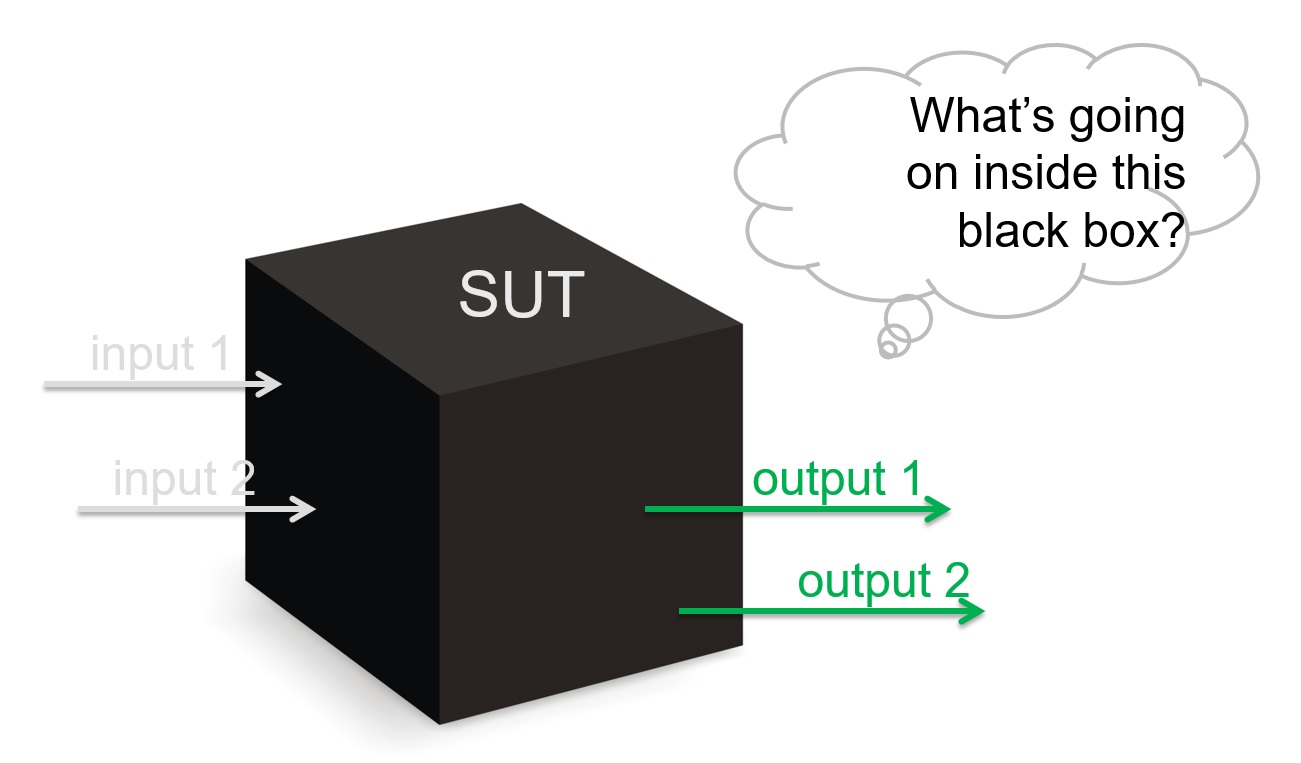
\includegraphics[width=.8\textwidth]{blackbox.jpg}
\end{center}
}

\frame{
\frametitle{Minimally adequate teacher (Angluin)}

\begin{center}
 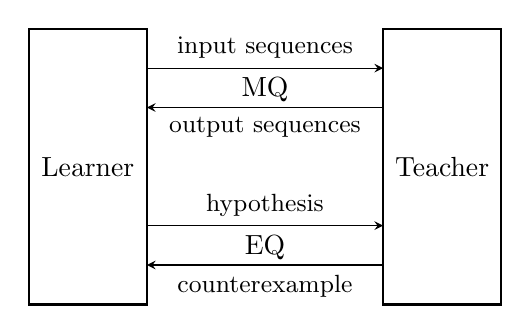
\begin{tikzpicture}[>=stealth]
            \draw [thick] (0,0) rectangle (1.5,3.5) node[midway] {Learner};
            \draw [thick] (4.5,0) rectangle (6,3.5) node[midway] {Teacher};
            \draw [->] (1.5,3) -- (4.5,3) node[midway,below] {MQ};
            \draw (1.5,3) -- (4.5,3) node[midway,above] {\small input sequences};
            \draw [<-] (1.5,2.5) -- (4.5,2.5) node[midway,below] {\small output sequences};
            \draw [->] (1.5,1) -- (4.5,1) node[midway,below] {EQ};
            \draw (1.5,1) -- (4.5,1) node[midway,above] {\small hypothesis};
            \draw [<-] (1.5,0.5) -- (4.5,0.5) node[midway,below] {\small counterexample};
        \end{tikzpicture}
        \hspace{2 em}
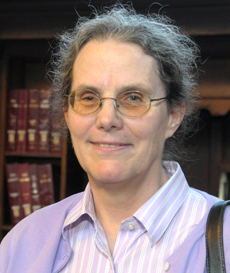
\includegraphics[width=.25\textwidth]{angluin.png}
\end{center}
}
\frame{
\frametitle{Black box checking (Peled, Vardi \& Yannakakis)}

\begin{center}
 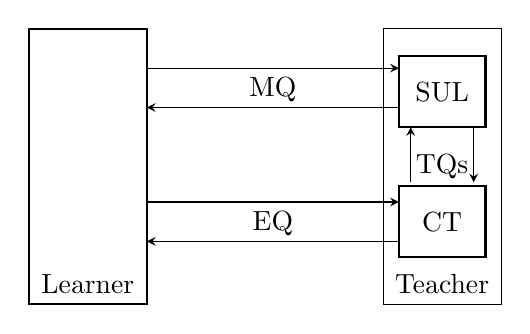
\begin{tikzpicture}[>=stealth]
            \draw [thick] (0,0) rectangle (1.5,3.5);
            \draw (4.5,0) rectangle (6,3.5) node[midway] {TQs};
            \draw [thick] (4.7,2.25) rectangle (5.8,3.15) node[midway] {SUL};
            \draw [thick] (4.7,0.6) rectangle (5.8,1.5) node[midway] {CT};
            \draw [->] (1.5,3) -- (4.7,3) node[midway,below] {MQ};
            \draw [<-] (1.5,2.5) -- (4.7,2.5);
            \draw [->] (1.5,1.3) -- (4.7,1.3) node[midway,below] {EQ};
            \draw [<-] (1.5,0.8) -- (4.7,0.8);
            \draw [->] (4.85,1.55) -- (4.85,2.25);
            \draw [<-] (5.65,1.55) -- (5.65,2.25);
            \node [below] at (0.75,0.5) {Learner};
            \node [below] at (5.25,0.5) {Teacher};
        \end{tikzpicture}
                \hspace{1 em}
        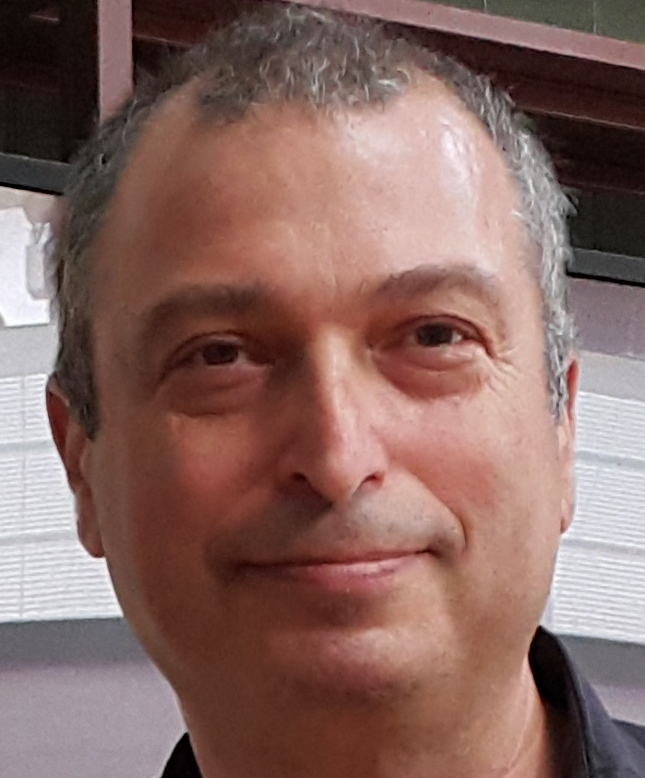
\includegraphics[width=1.2cm]{peled.jpg}
        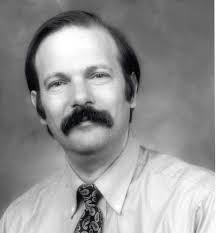
\includegraphics[width=1.35cm]{vardi.jpeg}
        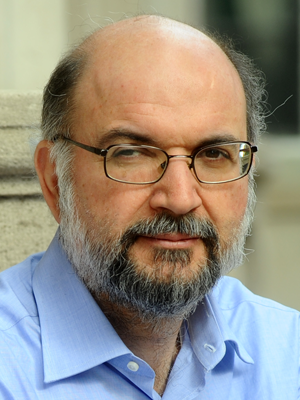
\includegraphics[width=1.1cm]{Yannakakis.png}
\end{center}
\red{Learner}: Formulate hypotheses\\
\red{Conformance Tester (CT)}: Test correctness hypotheses
}

\frame{
\frametitle{LearnLib}

\begin{center}

\includegraphics[width=.7\textwidth]{LearnLib.jpg}
    \hspace{1 em}
        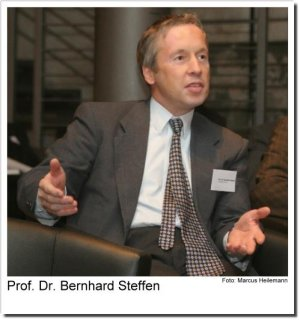
\includegraphics[width=2.5cm]{steffen.jpg}
\end{center}
}

\frame{
\frametitle{Research method}

\begin{center}
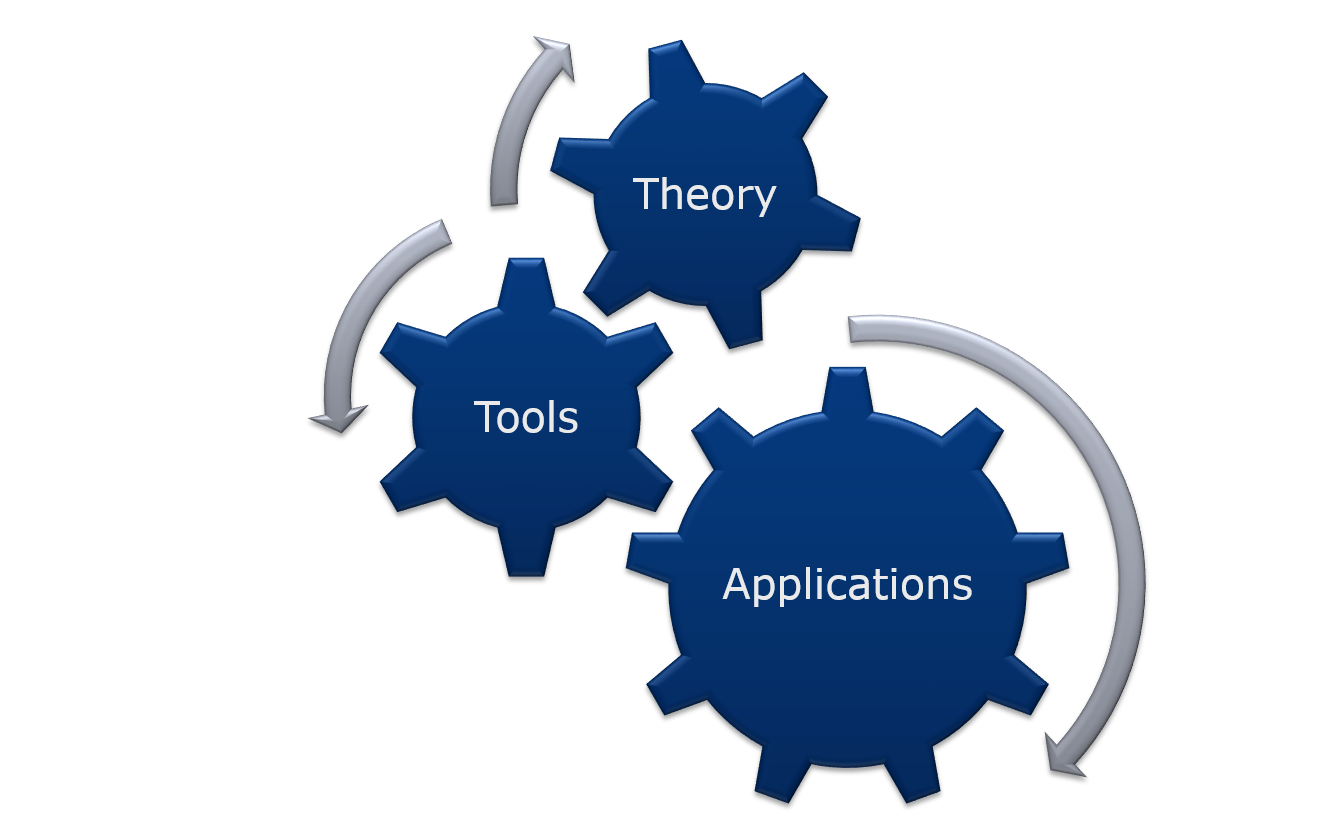
\includegraphics[width=.8\textwidth]{method.png}
\end{center}
\pause
This talk: \red{THEORY}\  
\pause
(motivated by earlier applications)
}

%\frame{
%\frametitle{Application: E.dentifier2}
%\begin{center}
%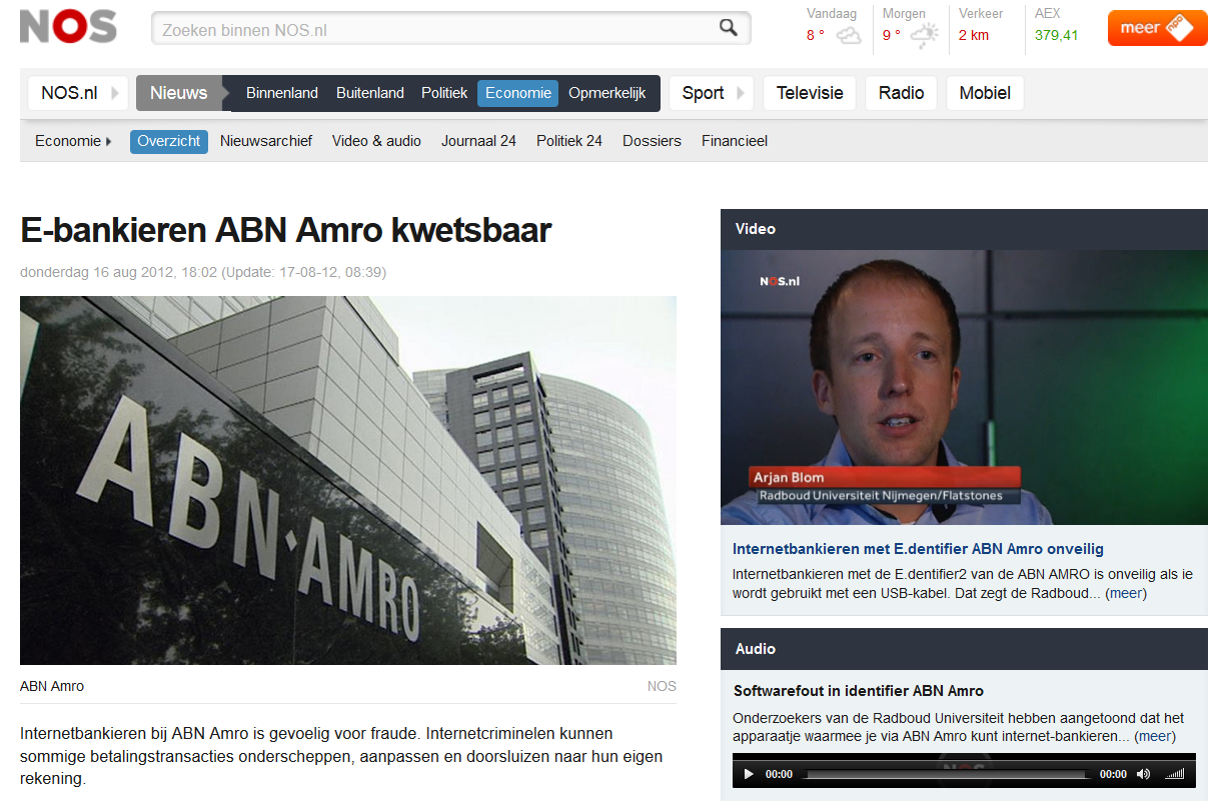
\includegraphics[width=.8\textwidth]{nosedentifier.png}
%\end{center}
%}

%\frame{
%\frametitle{State machines for old and new E.dentifier2}
%\begin{center}
%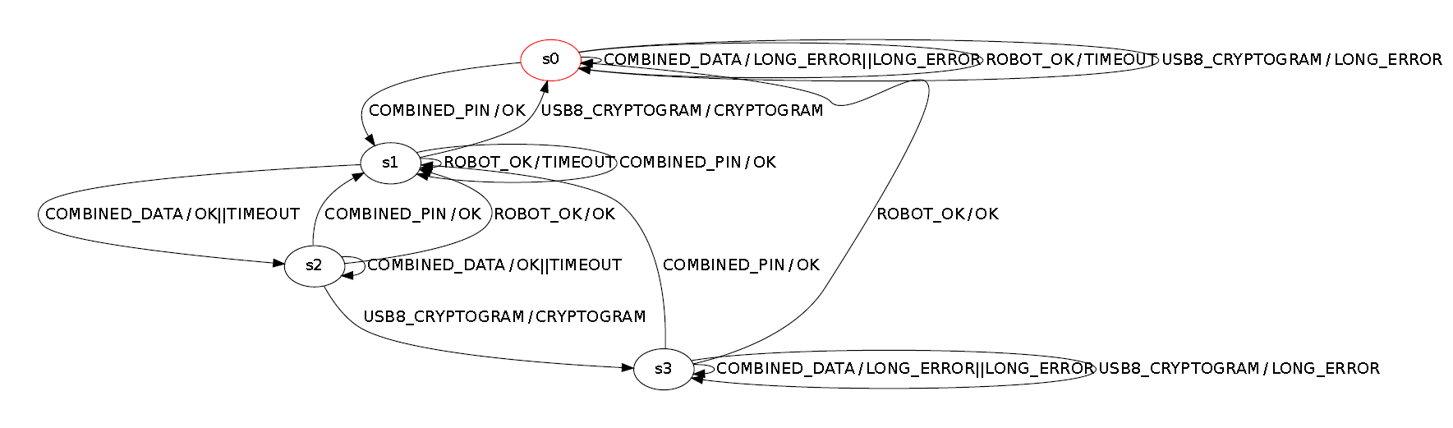
\includegraphics[width=.9\textwidth]{oldedentifier.png}
%
%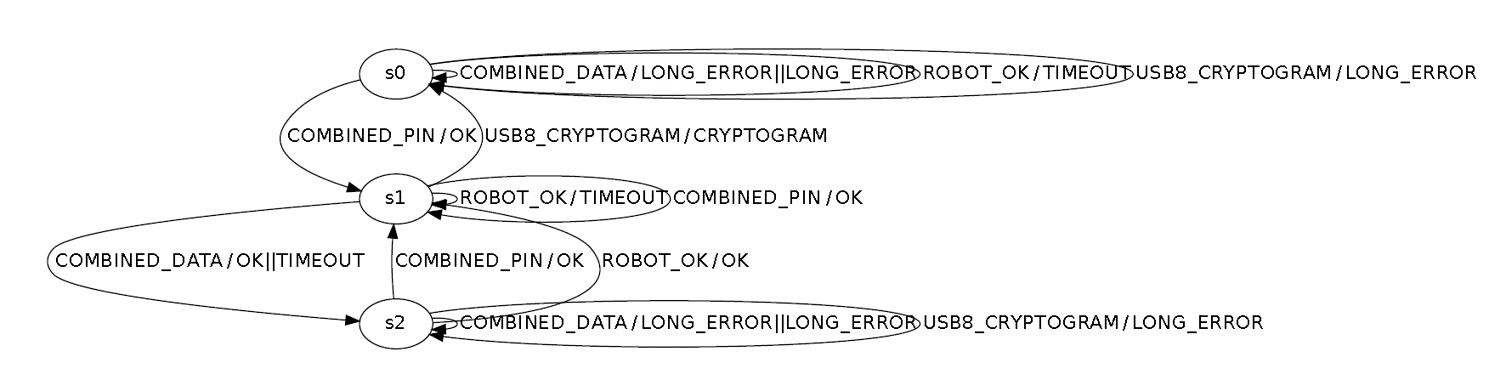
\includegraphics[width=.9\textwidth]{newedentifier.png}
%\end{center}
%}

\frame{
\frametitle{Bugs in protocol implementations}

\begin{center}
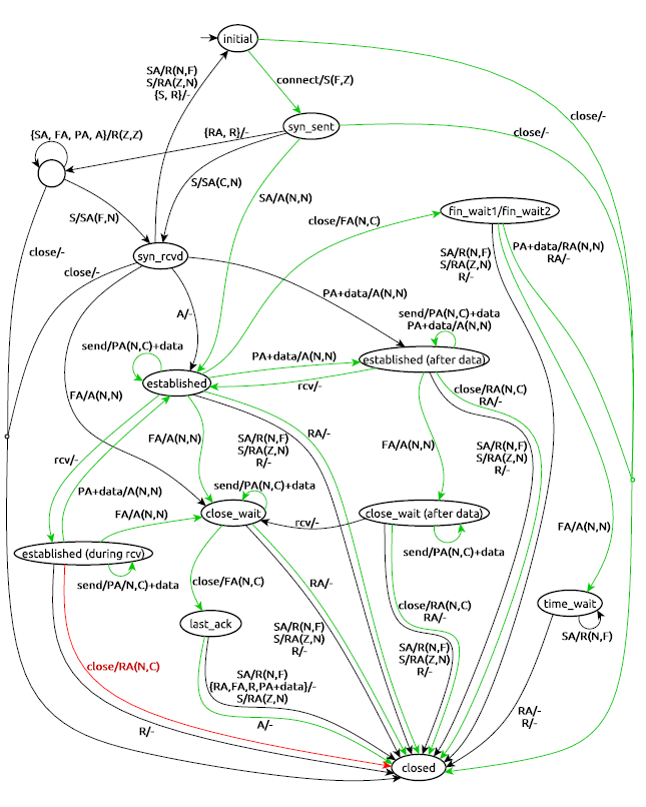
\includegraphics[width=.35\textwidth]{TCPbug.png}
\end{center}
{\small Standard violations found in implementations of major protocols, e.g.,
\blue{TCP}\  (CAV'16, FMICS'17), \blue{TLS}\  (Usenix Security'15), \blue{SSH}\  (Spin'17).}
%
\pause
\red{These findings led to several bug fixes in implementations.}
}

\frame{
\frametitle{Learned model for SSH implementation}

\begin{center}
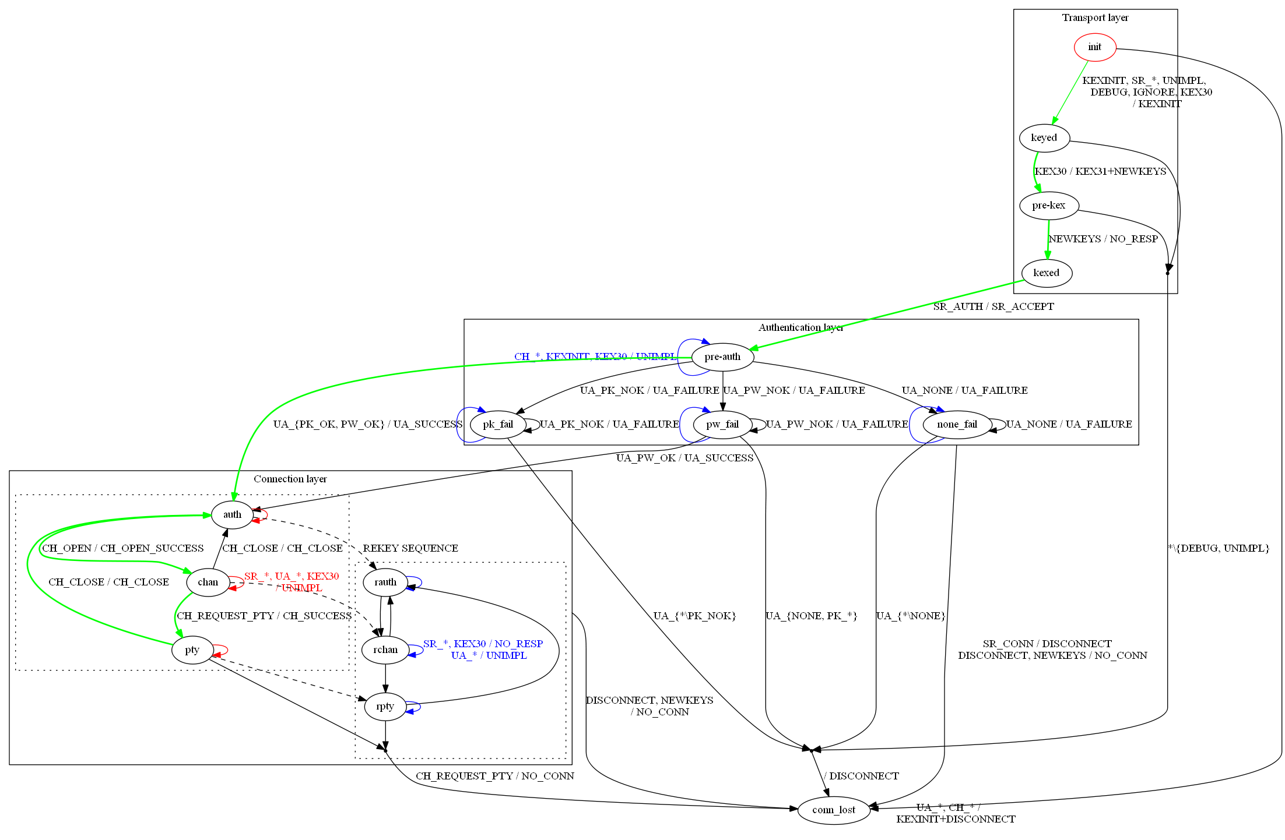
\includegraphics[width=.8\textwidth]{sshbug.png}
\end{center}
}

\frame{
\frametitle{SSH model checking results}

\begin{center}
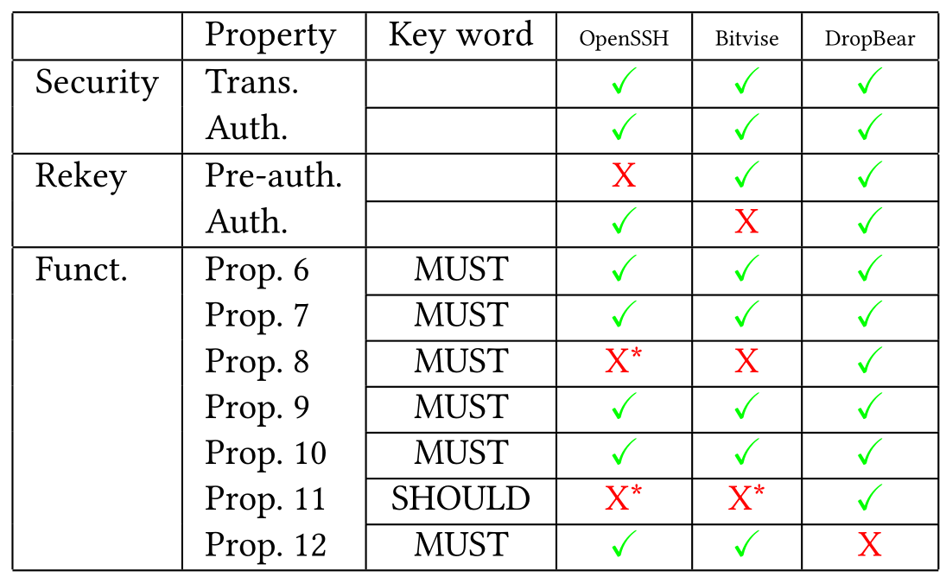
\includegraphics[width=.8\textwidth]{sshresults.png}
\end{center}
}

\frame{
\frametitle{For background and applications see CACM review article}

\begin{center}

\includegraphics[width=.4\textwidth]{cacm.jpg}
\end{center}
}

\frame{
\frametitle{Motivation for work presented today}

\blue{Timing behavior}\  plays a crucial role in applications of model learning, but existing algorithms and tools cannot handle it. 
%Today's tools only work for untimed, deterministic systems. \\

There is some work on algorithms for learning timed systems:
\begin{itemize}
\item
Grinchtein, Jonsson \& Leucker.\\ \green{Learning of event-recording automata}. TCS, 2010.
\item
Mens \& Maler.\\ \green{Learning Regular Languages over Large Ordered Alphabets}. LMCS, 2015.
\item
Caldwel, Cardell-Oliver \& French.\\ \green{Learning time delay Mealy machines}. IEEE TASE, 2016.
\end{itemize}
but this is not so practical because of high complexity and/or limited expressivity.
}

\section{Mealy machines with timers}
\frame{
\frametitle{Timing Behavior in Network Protocols}
Sender alternating-bit protocol, adapted from Kurose \& Ross, \green{Computer Networking}:

%\vspace{1em}
\begin{center}
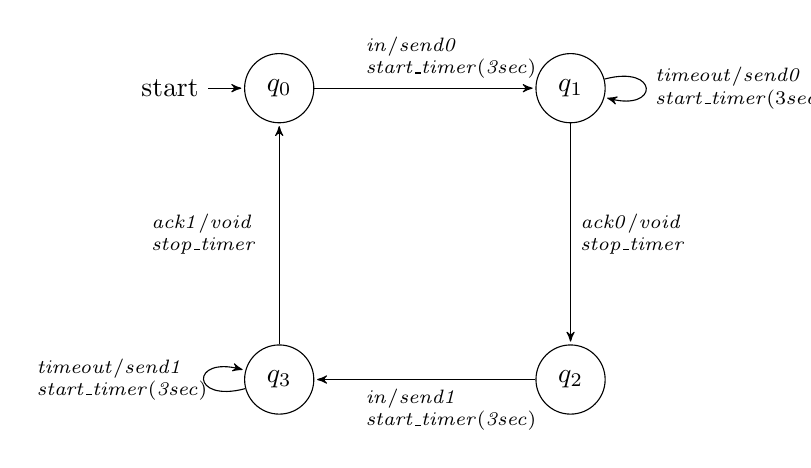
\begin{tikzpicture}[->,>=stealth',shorten >=1pt,auto,node distance=3.7cm,main node/.style={circle,draw,font=\sffamily\large\bfseries}]
  \node[initial, state] (1) {$q_0$};
  \node[state] (2) [right of=1] {$q_1$};
  \node[state] (3) [below of=2] {$q_2$};
  \node[state] (4) [below of=1] {$q_3$};

  \path[every node/.style={font=\sffamily\scriptsize}]
    (1) edge [text width=1.5cm] node {$\mathit{in}/\mathit{send0}$ \\ $\mathit{start\_timer(3sec)}$} (2)
    (2) edge [text width=1.5cm] node {$\mathit{ack0}/\mathit{void}$ \\ $\mathit{stop\_timer}$} (3)
        edge [loop right, text width=1.5cm] node {$\mathit{timeout}/\mathit{send0}$\\ $\mathit{start\_timer}(3sec)$ } (2)
    (3) edge [text width=1.5cm] node {$\mathit{in}/\mathit{send1}$ \\ $\mathit{start\_timer(3sec)}$} (4)
    (4) edge [text width=1.5cm] node {$\mathit{ack1}/\mathit{void}$ \\ $\mathit{stop\_timer}$} (1)
        edge [loop left, text width=2cm] node {$\mathit{timeout}/\mathit{send1}$\\ $\mathit{start\_timer(3sec)}$} (4);
\end{tikzpicture}
\end{center}
}

\frame{
\frametitle{Idea}

Develop learning algorithm for Mealy machines with timers!!!
% in which transitions can be triggered by both input events and timeouts,
%and may start, stop and restart multiple timers.

\vspace{2 em}
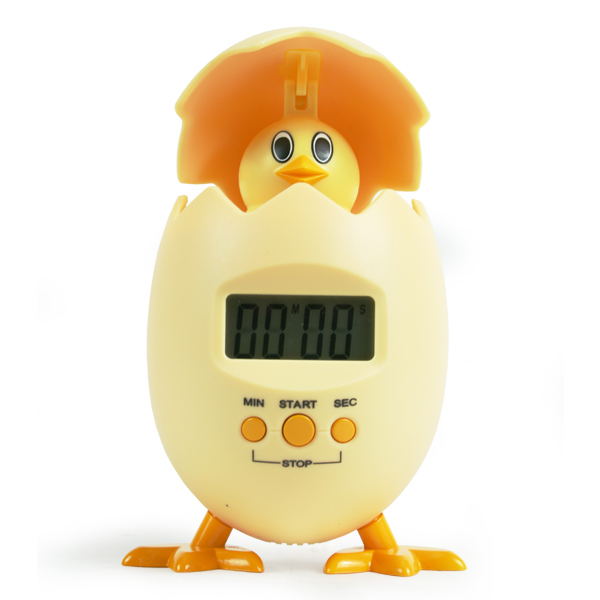
\includegraphics[width=.2\textwidth]{egg_timer0.jpg}
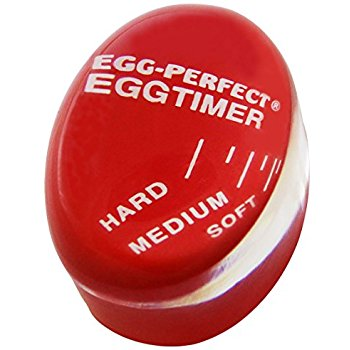
\includegraphics[width=.2\textwidth]{egg_timer2.jpg}
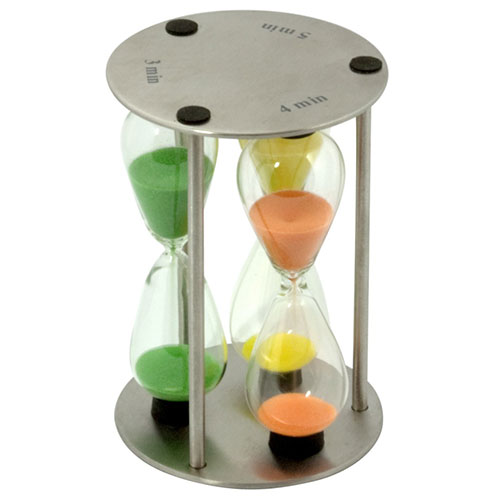
\includegraphics[width=.2\textwidth]{Sand-timer.jpg}
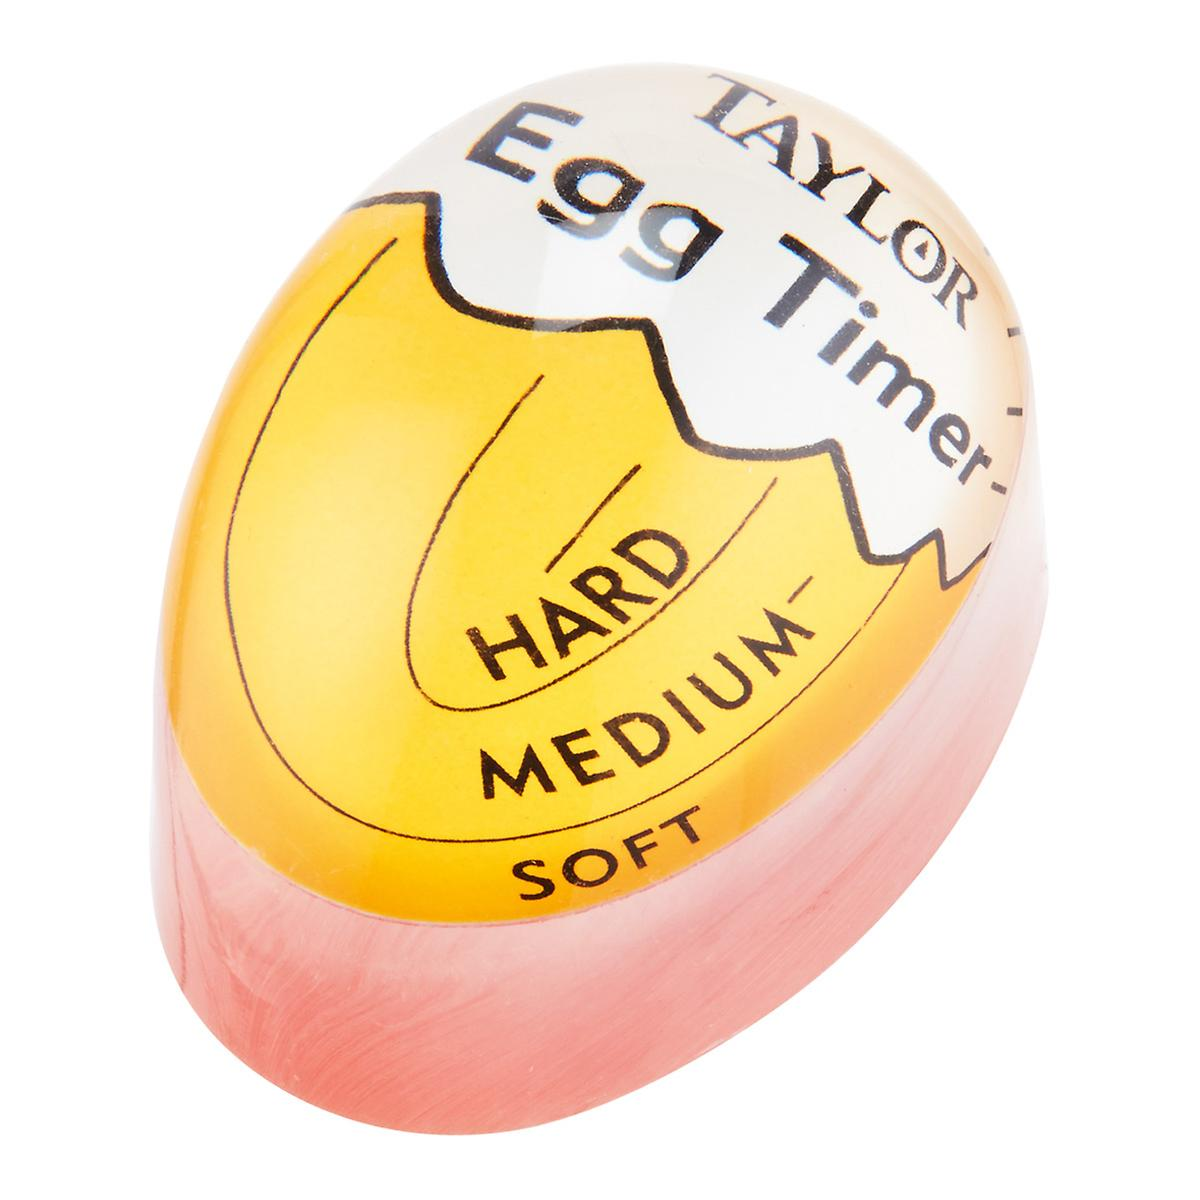
\includegraphics[width=.2\textwidth]{egg_timer3.jpg}
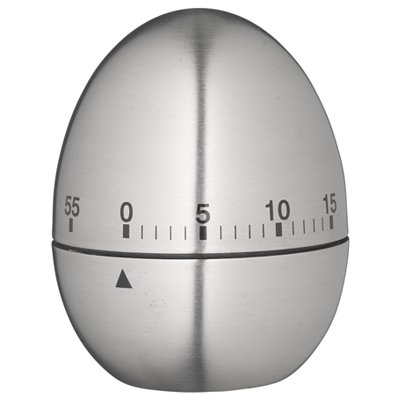
\includegraphics[width=.2\textwidth]{egg_timer4.jpg}

\pause
\vspace{2 em}
\blue{\em Occurrence of timing dependent behavior fully determined by previous behavior}
}


\frame{
\frametitle{MMTs}
Assume an unbounded set $X$ of {\red{timers}}\  $x$, $x_1$, $x_2$, etc.\ 
%
For a set $I$,  write $\extinputs = I \cup \{ \toevent{x} \mid x \in X \}$.

\begin{block}{Definition}
A \red{Mealy machine with timers (MMT)}\  is a tuple
$\M = (I, O, Q, q_0, \vars, \delta, \lambda, \remap)$, where
\begin{itemize}
\item
$I$ and $O$ are finite sets of input and output events
\item
$Q$ is a finite set of states
with
$q_0 \in Q$ the initial state
\item
$\vars: Q \rightarrow \finitesubsets{X}$, with $\varsof{q_0} = \emptyset$
\item
$\delta: Q \times \extinputs \hookrightarrow  Q$ is a transition function,
%with $\delta(q,i)$ defined iff $q \in Q$ and $i \in I \cup \{ \toevent{x} \mid x \in \varsof{q} \}$, 
\item
$\lambda: Q \times \extinputs \hookrightarrow O$ is an output function,
\item
$\remap : Q \times \extinputs \hookrightarrow (X \hookrightarrow \natplus)$ is a timer update function
\end{itemize}
(satisfying some natural conditions)
\end{block}
}

\frame{
\frametitle{Operations on timers}
Write $q \xrightarrow{i/o,\rho} q'$ if $\delta(q,i) = q'$, $\lambda(q,i)= o$ and $\remap(q,i) = \rho$.

Basically, four things can happen:

\begin{enumerate}
\item
If $x \in\varsof{q} \setminus \varsof{q'}$ then input $i$ \red{stops}\  timer $x$.
\item
If $x \in \varsof{q'} \setminus \varsof{q}$ then $i$ \red{starts}\  timer $x$ with value $\rho(x)$.
\item
If $x \in \varsof{q} \cap \domof{\rho}$ then $i$ \red{restarts}\  timer $x$ with value $\rho(x)$.
\item
Finally, if $x \in \varsof{q'} \setminus \domof{\rho}$ then timer $x$ is \red{unaffected}\  by $i$.
\end{enumerate}
}

\frame{
\frametitle{Timed Semantics (1)}
A \red{configuration}\  of an MMT is a pair $(q, \tvals)$ of a state $q$ and a valuation $\tvals : \varsof{q} \rightarrow \realsplus$ of its timers.
When time advances, all timers decrease at the same rate; a timeout occurs when value of some timer becomes $0$.

\vspace{1 em}
A \red{timed run}\  of an MMT is a sequence 
\[
(q_0, \tvals_0) \xrightarrow{d_1} (q_0, \tvals'_0) \xrightarrow{i_1/o_1} (q_1, \tvals_1) \xrightarrow{d_2} \cdots
 \xrightarrow{i_k/o_k} (q_k, \tvals_k)
\]
of configurations, \blue{nonzero}\  delays, and discrete transitions.
}


\frame{
\frametitle{Timed Semantics (2)}

A \red{timed word}\   describes an observation we can make on an MMT:
\begin{eqnarray*}
w & = &  d_1 ~ i_1 ~ o_1 ~ d_2 ~ i_2 ~ o_2 \cdots d_k ~ i_k ~ o_k,
\end{eqnarray*}
where $d_j \in \delays$, $i_j \in I \cup \{ \mathit{to} \}$, and $o_j \in O$.

\vspace{1 em}
To each timed run $\alpha$ we associate a timed word \red{$\timedword(\alpha)~$} by forgetting the configurations and names of timers
in timeouts.

\vspace{1 em}
\begin{block}{Definition}
MMTs $\M$ and $\N$ are \red{timed equivalent}, denoted $\M \approx_{\mathit{timed}} \N$, iff 
they have the same timed words.
\end{block}
}

\frame{
\frametitle{``Uncontrollable'' Nondeterminism}

\begin{center}
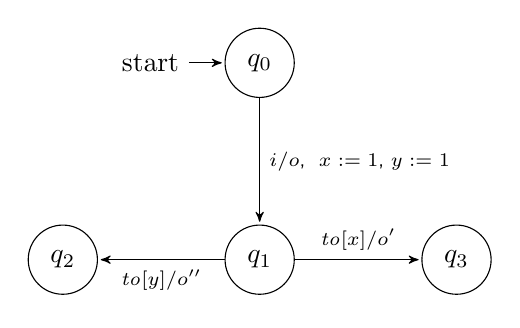
\begin{tikzpicture}[->,>=stealth',shorten >=1pt,auto,node distance=2.5cm,main node/.style={circle,draw,font=\sffamily\large\bfseries}]
  \node[initial, state] (1) {$q_0$};
  \node[state] (2) [below of=1] {$q_1$};
  \node[state] (3) [right of=2] {$q_3$};
  \node[state] (4) [left of=2] {$q_2$};

  \path[every node/.style={font=\sffamily\scriptsize}]
    (1) edge node {$i/o$, $~x:=1$, $y:=1$} (2)  
    (2) edge  node {$\toevent{x}/o'$} (3)
     edge  node {$\toevent{y}/o''$} (4);
\end{tikzpicture}
\end{center}

Accepts timed words
$1 ~ i ~ o ~ 1 ~ \mathit{to} ~ o'$ and $1 ~ i ~ o ~ 1 ~ \mathit{to} ~ o''$.

\pause
\vspace{1 em}
$\Rightarrow$ \blue{We assume at most one timer can be updated per transition.}
}

\frame{
\frametitle{``Controllable'' Nondeterminism}


\begin{center}
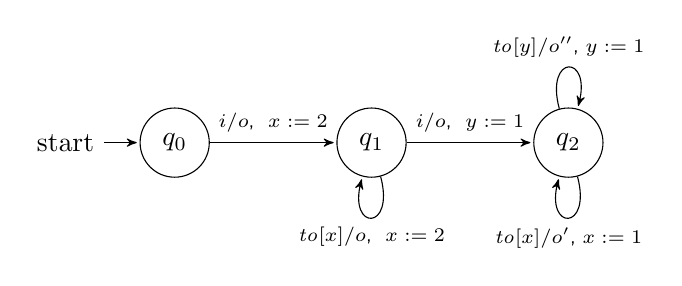
\begin{tikzpicture}[->,>=stealth',shorten >=1pt,auto,node distance=2.5cm,main node/.style={circle,draw,font=\sffamily\large\bfseries}]
  \node[initial, state] (1) {$q_0$};
  \node[state] (2) [right of=1] {$q_1$};
  \node[state] (3) [right of=2] {$q_2$};

  \path[every node/.style={font=\sffamily\scriptsize}]
    (1) edge node {$i/o$, $~x:=2$} (2)  
    (2) edge  node {$i/o$, $~y:=1$} (3)
      edge  [loop below] node {$\toevent{x}/o$, $~x:=2$} (2)
   (3) edge  [loop below] node {$\toevent{x}/o'$, $x:=1$} (3)
   edge  [loop above] node {$\toevent{y}/o''$, $y:=1$} (3);
\end{tikzpicture}
\end{center}

Accepts timed words $7 ~ i ~ o ~ 1 ~ i ~ o ~ 1 ~ \mathit{to} ~ o'$ and $7 ~ i ~ o ~ 1 ~ i ~ o ~ 1 ~ \mathit{to} ~ o''$.

\pause
\vspace{1 em}
$\Rightarrow$ \blue{During learning we will simply avoid these race conditions.}
}

\frame{
\frametitle{A timed MAT framework}

{\small
A \red{timed input word}\  is a sequence
$u = d_1 ~ i_1 \cdots d_k ~ i_k ~ d_{k+1}$, with $d_j \in \delays$ and $i_j \in I$, for  $j \leq k$,
and $d_{k+1} \in \realsplus$.
%
%To each timed word $w$ we associate a timed input word \red{$\timedinputword(w)$}.
%
%Write \red{$u \propto u'$}\  if $u$ and $u'$ are equal, except that final delay of $u$ may be less or equal than final delay of $u'$.
A timed (input) word is \red{transparent}\  if inputs occur at different fractional times. 
}

\begin{center}
 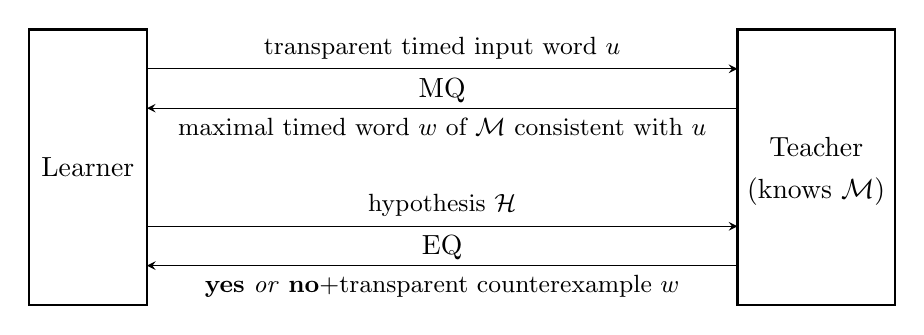
\begin{tikzpicture}[>=stealth]
            \draw [thick] (0,0) rectangle (1.5,3.5) node[midway] {Learner};
            \draw [thick] (9,0) rectangle (11,3.5) node[midway,above] {Teacher};
            \draw [thick] (9,0) rectangle (11,3.5) node[midway,below] {(knows $\M$)};
            \draw [->] (1.5,3) -- (9,3) node[midway,below] {MQ};
            \draw (1.5,3) -- (9,3) node[midway,above] {\small transparent timed input word $u$};
            \draw [<-] (1.5,2.5) -- (9,2.5) node[midway,below] {\small maximal timed word $w$ of $\M$ consistent with $u$};
            \draw [->] (1.5,1) -- (9,1) node[midway,below] {EQ};
            \draw (1.5,1) -- (9,1) node[midway,above] {\small hypothesis $\CH$};
            \draw [<-] (1.5,0.5) -- (9,0.5) node[midway,below] {\small {\bf yes} \emph{or} {\bf no}+transparent counterexample $w$};
        \end{tikzpicture}
\end{center}  
\pause
\blue{Main contribution: algorithm allowing learner to construct MMT $\N$ that is timed equivalent to $\M$ (under mild restrictions).}    
}

\frame{
\frametitle{Plan of attack}

\begin{center}
 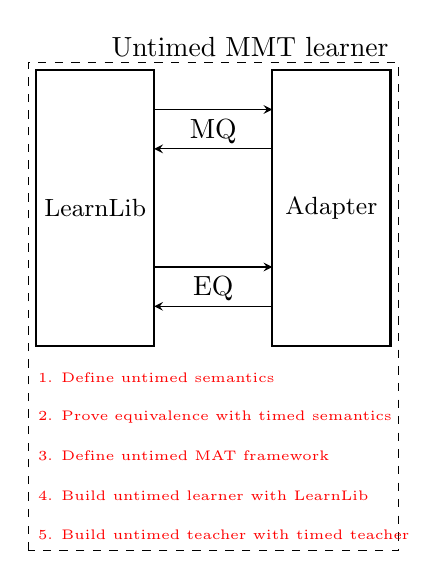
\begin{tikzpicture}[>=stealth]
 \draw [dashed] (-0.1,-2.6) rectangle (4.6,3.6);
 \node[above, left] at (4.6,3.8) {Untimed MMT learner};
            \draw [thick] (0,0) rectangle (1.5,3.5) node[midway] {\small LearnLib};
            \draw [thick] (3,0) rectangle (4.5,3.5) node[midway] {\small Adapter};
            \draw [->] (1.5,3) -- (3,3) node[midway,below] {MQ};
            \draw [<-] (1.5,2.5) -- (3,2.5);
            \draw [->] (1.5,1) -- (3,1) node[midway,below] {EQ};
            \draw [<-] (1.5,0.5) -- (3,0.5);
            \node[right, red] at (-0.1,-0.4) {\tiny 1. Define untimed semantics};
            \node[right, red] at (-0.1,-0.9) {\tiny 2. Prove equivalence with timed semantics};
            \node[right, red] at (-0.1,-1.4) {\tiny 3. Define untimed MAT framework};
            \node[right, red] at (-0.1,-1.9) {\tiny 4. Build untimed learner with LearnLib};
            \node[right, red] at (-0.1,-2.4) {\tiny 5. Build untimed teacher with timed teacher};
            %\draw [->] (4.5,3) -- (5.5,3);
            %\draw [<-] (4.5,2.5) -- (5.5,2.5);
            %\draw [->] (4.5,1) -- (5.5,1);
           % \draw [<-] (4.5,0.5) -- (5.5,0.5);
        \end{tikzpicture}
        \hspace{-0.4cm}
 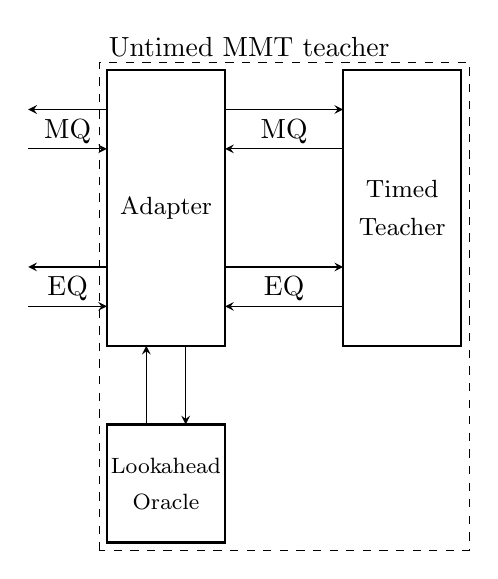
\begin{tikzpicture}[>=stealth]
 \draw [dashed] (-0.1,-2.6) rectangle (4.6,3.6);
 \node [above,right] at (-0.1,3.8) {Untimed MMT teacher};
            \draw [thick] (0,0) rectangle (1.5,3.5) node[midway] {\small Adapter};
            \draw [thick] (3,0) rectangle (4.5,3.5) node[midway,above] {\small Timed}; 
            \draw [thick] (3,0) rectangle (4.5,3.5) node[midway,below] {\small Teacher};
            \draw [->] (1.5,3) -- (3,3) node[midway,below] {MQ};
            \draw [<-] (1.5,2.5) -- (3,2.5);
            \draw [->] (1.5,1) -- (3,1) node[midway,below] {EQ};
            \draw [<-] (1.5,0.5) -- (3,0.5);
            \draw [->] (0,3) -- (-1,3) node[midway,below] {MQ};
            \draw [<-] (0,2.5) -- (-1,2.5);
            \draw [->] (0,1) -- (-1,1) node[midway,below] {EQ};
            \draw [<-] (0,0.5) -- (-1,0.5);
            \draw [thick] (0,-2.5) rectangle (1.5,-1) node[midway,below] {\footnotesize Oracle};
            \draw [thick] (0,-2.5) rectangle (1.5,-1) node[midway,above] {\footnotesize Lookahead};
            \draw [->] (0.5,-1) -- (0.5,0); % node[midway,left] {\small {\bf no} \emph{or} {\bf yes}+timeout value};
            \draw [->] (1,0) -- (1,-1); % node[midway,right] {\small untimed input word $u$ + index $j$};
        \end{tikzpicture}
\end{center}

}

\frame{
\frametitle{Timed and Untimed Runs and Behaviors}
\begin{center}
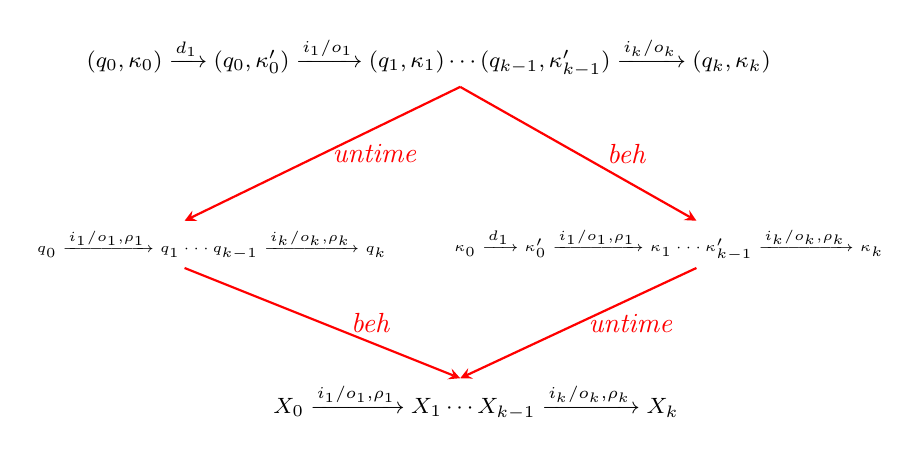
\begin{tikzpicture}[>=stealth]
\node [above] at (5.1,4) {\footnotesize ($q_0, \tvals_0) \xrightarrow{d_1} (q_0, \tvals'_0) \xrightarrow{i_1/o_1} (q_1, \tvals_1)  \cdots
(q_{k-1}, \tvals'_{k-1}) \xrightarrow{i_k/o_k} (q_k, \tvals_k)$};
%An \red{untimed run}\  of an MMT $\M$ is a sequence
\node [right] at (0,2) {\tiny $q_0 \xrightarrow{i_1/o_1, \rho_1} q_1  \cdots q_{k-1} \xrightarrow{i_k/o_k, \rho_k} q_k$};
%A \red{timed behavior}\  is a sequence
\node [left] at (11,2) {\tiny $\tvals_0 \xrightarrow{d_1} \tvals'_0 \xrightarrow{i_1/o_1, \rho_1} \tvals_1  \cdots \tvals'_{k-1} \xrightarrow{i_k/o_k, \rho_k} \tvals_{k}$};
%An \red{untimed behavior}\  is a sequence 
\node at (5.7,0) {\footnotesize $X_0 \xrightarrow{i_1/o_1, \rho_1} X_1  \cdots X_{k-1} \xrightarrow{i_k/o_k, \rho_k} X_{k}$};
\draw [thick, red, ->] (5.5,4) -- (2,2.3) node[midway, right] {$\untime$};
\draw [thick, red, ->] (5.5,4) -- (8.5,2.3) node[midway, right] {$~~\beh$};
\draw [thick, red, ->] (8.5,1.7) -- (5.5,0.3) node[midway, right] {$\untime$};
\draw [thick, red, ->] (2,1.7) -- (5.5,0.3) node[midway, right] {$~~\beh$};
\end{tikzpicture}
\end{center}
}

\frame{
\frametitle{Timed and Untimed Runs and Behaviors}

Diagram commutes and has a \blue{pullback}:
\begin{center}
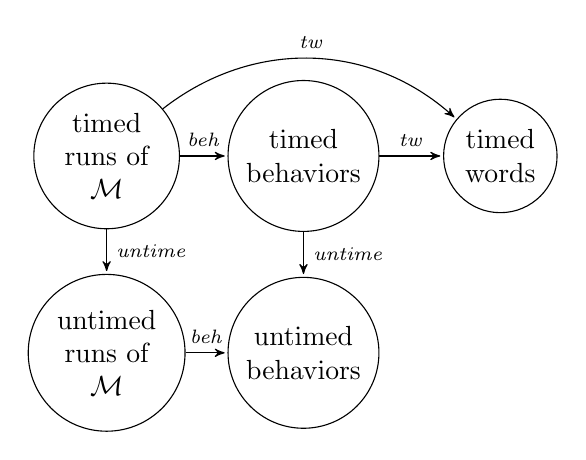
\begin{tikzpicture}[->,>=stealth',shorten >=1pt,auto,node distance=2.5cm,main node/.style={circle,draw,font=\sffamily\large\bfseries}]
  \node[state,align=center] (1) {timed \\ runs of\\ $\M$};
  \node[state,align=center] (2) [below of=1] {untimed \\ runs of\\ $\M$};
  \node[state,align=center] (3) [right of=1] {timed\\ behaviors};
  \node[state,align=center] (4) [right of=2] {untimed\\ behaviors};
  \node[state,align=center] (5) [right of=3] {timed \\words};

  \path[every node/.style={font=\sffamily\scriptsize}]
    (1) edge  node {$\untime$} (2)
        edge  node {$\beh$} (3)
        edge[bend left=40]  node {$\timedword$} (5)
    (2) edge  node {$\beh$} (4)
    (3) edge  node {$\untime$} (4)
        edge  node {$\timedword$} (5);
\end{tikzpicture}
\pause
\red{\small
\begin{tabular}{l}
CAN WE DEFINE\\
SEMANTICS MMTs\\
IN TERMS OF\\
UNTIMED\\ BEHAVIORS??
\end{tabular}
}
\end{center}
}

\section{Untimed semantics}
\frame{
\frametitle{Feasibility}

\begin{block}{Definition}
An untimed behavior 
\[
\beta ~=~ X_0 \xrightarrow{i_1/o_1, \rho_1} X_1  \xrightarrow{i_2/o_2, \rho_2} X_2 \cdots \xrightarrow{i_k/o_k, \rho_k} X_{k}
\]
is \red{feasible}\ if there is a timed behavior $\sigma$ such that $\untime(\sigma) = \beta$.
\end{block}

\vspace{1 em}
Example of  untimed behavior that is \emph{not} feasible: 
\[
\emptyset \xrightarrow{i_1/o_1, x:=1} \{ x \}  \xrightarrow{i_2/o_2, y:=100} \{ x, y \} \xrightarrow{\toevent{y} /o_3} \emptyset
\]
}

\frame{
\frametitle{Untimed semantics}

\begin{block}{Definition}
MMTs $\M$ and $\N$ are \red{untimed equivalent}, $\M \approx_{\mathit{untimed}} \N$, iff their sets of feasible untimed behaviors are \red{isomorphic}, that is, equal modulo renaming of timers.
\end{block}

\pause
\vspace{1 em}
\begin{block}{Theorem}
$\M \approx_{\mathit{untimed}} \N$
implies
$\M \approx_{\mathit{timed}} \N$.
\end{block}

\pause
Converse implication does not hold in general.
}

\iflong
\frame{
\frametitle{Starting multiple timers on one transition}

Timed equivalent but not untimed equivalent:

\vspace{1 em}
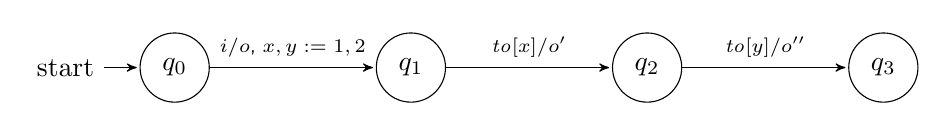
\begin{tikzpicture}[->,>=stealth',shorten >=1pt,auto,node distance=3cm,main node/.style={circle,draw,font=\sffamily\large\bfseries}]
  \node[initial, state] (1) {$q_0$};
  \node[state] (2) [right of=1] {$q_1$};
  \node[state] (3) [right of=2] {$q_2$};
  \node[state] (4) [right of=3] {$q_3$};

  \path[every node/.style={font=\sffamily\scriptsize}]
    (1) edge node {$i/o$, $x, y:=1,2$} (2)  
    (2) edge  node {$\toevent{x}/o'$} (3)
   (3) edge node {$\toevent{y}/o''$} (4);
\end{tikzpicture}

\vspace{2 em}
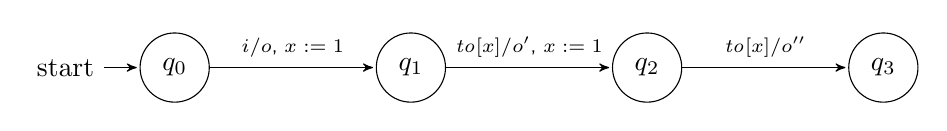
\begin{tikzpicture}[->,>=stealth',shorten >=1pt,auto,node distance=3cm,main node/.style={circle,draw,font=\sffamily\large\bfseries}]
  \node[initial, state] (1) {$q_0$};
  \node[state] (2) [right of=1] {$q_1$};
  \node[state] (3) [right of=2] {$q_2$};
  \node[state] (4) [right of=3] {$q_3$};

  \path[every node/.style={font=\sffamily\scriptsize}]
    (1) edge node {$i/o$, $x:=1$} (2)  
    (2) edge  node {$\toevent{x}/o'$, $x:=1$} (3)
   (3) edge node {$\toevent{x}/o''$} (4);
\end{tikzpicture}

\pause
\vspace{1 em}
$\Rightarrow$ \blue{We assume at most one timer can be updated per transition.}

\pause
\vspace{1 em}
This also eliminates ``uncontrollable'' nondeterminism! 
%For most MMTs there is equivalent MMT that updates at most
%one timer per transition.
}
\fi

\frame{
\frametitle{Ghost timers}

\begin{center}
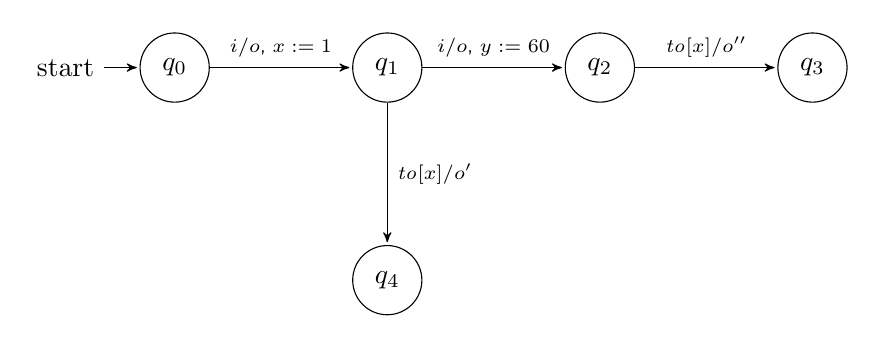
\begin{tikzpicture}[->,>=stealth',shorten >=1pt,auto,node distance=2.7cm,main node/.style={circle,draw,font=\sffamily\large\bfseries}]
  \node[initial, state] (1) {$q_0$};
  \node[state] (2) [right of=1] {$q_1$};
  \node[state] (3) [right of=2] {$q_2$};
  \node[state] (4) [right of=3] {$q_3$};
  \node[state] (5) [below of=2] {$q_4$};

  \path[every node/.style={font=\sffamily\scriptsize}]
    (1) edge node {$i/o$, $x:=1$} (2)  
    (2) edge  node {$i/o$, $y:=60$} (3)
   (3) edge node {$\toevent{x}/o''$} (4)
   (2) edge node {$\toevent{x}/o'$} (5);
\end{tikzpicture}
\end{center}


}


\frame{
\frametitle{Equivalence of Timed and Untimed Semantics}
%\begin{block}{Definition}
%An MMTs $\M$ is \red{timer live}\  if for each feasible untimed behavior $\beta$ of $\M$ and each timer $y$ active after $\beta$, 
%there is a \red{witness}, a behavior $\beta_y$  that leaves $y$ unaffected, except for the last transition in which $y$ expires, such that %$\beta \cdot \beta_y$ is a feasible behavior of $\M$.
%\end{block}

%\pause

\begin{block}{Theorem}  
Suppose that $\M$ and $\N$ are MMTs without ghost timers in which at most one timer is started on each transition.\\
 Then
$\M \approx_{\mathit{timed}} \N$
implies
$\M \approx_{\mathit{untimed}} \N$.
\end{block}

\pause
\vspace{1 em}
Main proof technique: \blue{wiggling}\  of timed behaviors 
to ensure that fractional starting times of different inputs are different.
}

\iflong
\frame{
\frametitle{Wiggling}

\begin{center}
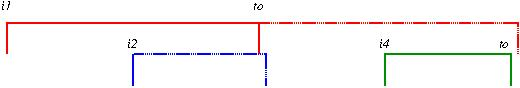
\includegraphics[width=.8\textwidth]{wiggling.jpg}
\end{center}

We partition all events in \red{blocks}\  that contains an input and all timeouts that it triggers.
A \red{race}\ occurs when right before an event some timer is $0$ and this event is not a timeout of that timer.

\pause
\begin{block}{Wiggle Lemmas}
\begin{enumerate}
\item
If there are no races we can wiggle any block
\item
Each race is won by one block
\item
A block can lose only once
\item
Blocks are partially ordered by winning relation
\item
A block that doesn't win any race can be wiggled forward
\end{enumerate}
\end{block}
}

\frame{
\frametitle{Retrieving causality}

A timed word is \red{transparent}\  if the fractional part of the absolute times of all inputs in $I$ is different. 

\begin{block}{Lemma}
Let $\sigma$ be any timed behavior.
Then there exists a timed behavior $\sigma'$ such that $\untime(\sigma)=\untime(\sigma')$ and $\timedword(\sigma')$ is transparent.
\end{block}

\pause
A \red{causality map}\  for timed word $w$ is an injective function that maps each timeout to a preceding event such that
the time elapsed between event and timeout is an integer.

\begin{block}{Lemma}
Suppose $\alpha$ is a timed run in which at most one timer is set
per transition, and $w =  \timedword(\alpha)$ is transparent. 
Then $w$ has a unique causality map.
\end{block}
}

\fi

\section{Learning algorithm}

\frame{
\frametitle{An untimed MAT framework}

{\small
An \red{untimed input word}\  is a sequence $u = i_1 \cdots i_k$ over $\extinputs$ such that
$i_j = \toevent{x_l}$ implies $l < j$, and each timer expires at most once.

\vspace{0.5em}
An untimed behavior $\beta$ is \red{canonical}\  if, for each $j$, the timer started in the $j$-th event (if any) is $x_j$.
%
%In this case, \red{$\untimedinputword(\beta)$}\  is the subsequence of inputs occurring in $\beta$.
%Each behavior $\beta$ is isomorphic to a canonical behavior.
}

\begin{center}
 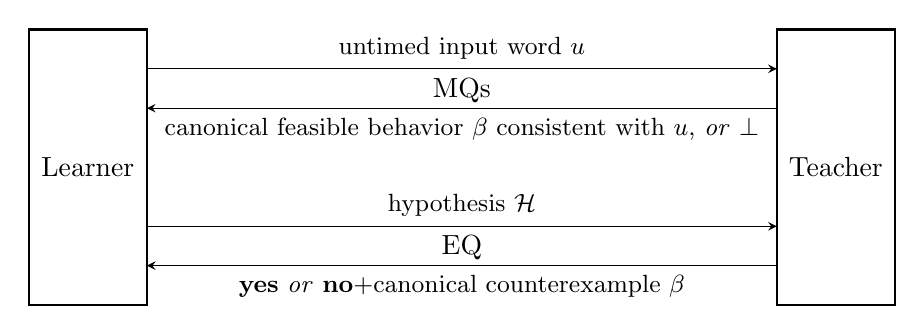
\begin{tikzpicture}[>=stealth]
            \draw [thick] (0,0) rectangle (1.5,3.5) node[midway] {Learner};
            \draw [thick] (9.5,0) rectangle (11,3.5) node[midway] {Teacher};
            \draw [->] (1.5,3) -- (9.5,3) node[midway,below] {MQs};
            \draw (1.5,3) -- (9.5,3) node[midway,above] {\small untimed input word $u$};
            \draw [<-] (1.5,2.5) -- (9.5,2.5) node[midway,below] {\small canonical feasible behavior $\beta$ consistent with $u$, \emph{or} $\perp$};
            \draw [->] (1.5,1) -- (9.5,1) node[midway,below] {EQ};
            \draw (1.5,1) -- (9.5,1) node[midway,above] {\small hypothesis $\CH$};
            \draw [<-] (1.5,0.5) -- (9.5,0.5) node[midway,below] {\small {\bf yes} \emph{or} {\bf no}+canonical counterexample $\beta$};
        \end{tikzpicture}
\end{center}        
}

\frame{
\frametitle{Myhill-Nerode (1)}

\begin{block}{Definition}
Let $S$ be a set of feasible untimed behaviors. Then $S$ is
\begin{itemize}
\item
\red{prefix closed}: $\beta \beta' \in S \Longrightarrow \beta \in S$,
\item
\red{behavior deterministic}:
$\beta \xrightarrow{i/o_1, \rho_1} X_1 \in S \wedge \beta \xrightarrow{i/o_2, \rho_2} X_2 \in S \Longrightarrow o_1 = o_2 \wedge \rho_1 = \rho_2 \wedge X_1 = X_2$,
\item
\red{input complete}:
$\beta \in S \wedge i \in I \Longrightarrow \exists o, \rho, Y : \beta \xrightarrow{i/o, \rho} Y \in S$,
\item
\red{timeout complete}:
$\beta \in S \wedge x \mbox{ expirable after } \beta \Longrightarrow
\exists o, \rho, Y: \beta \xrightarrow{\toevent{x}/o, \rho} Y \in S$.
\end{itemize}
Behaviors $\beta, \beta' \in S$ are \red{equivalent}, notation $\beta \equiv_S \beta'$, iff 
for any untimed behavior
$\gamma$, $\beta \cdot \gamma \in S \Leftrightarrow \beta' \cdot \gamma \in S$.
\end{block}
}

\frame{
\frametitle{Myhill-Nerode (2)}

\begin{block}{Theorem}
Let $S$ be a set of feasible untimed behaviors over finite sets of inputs $I$ and outputs $O$.
Then $S$ is the set of feasible untimed behaviors of an MMT $\M$ iff 
\begin{enumerate}
\item
$S$ is nonempty, 
\item
all behaviors in $S$ start with the empty set of timers, 
\item
the set of timers that occur in $S$ is finite, 
\item
$S$ is prefix closed, 
\item
$S$ is behavior deterministic, 
\item
$S$ is input complete, 
\item
$S$ is timeout complete, and 
\item
$\equiv_S$ has only finitely many equivalence classes (finite index).
\end{enumerate}
\end{block}
}

\frame{
\frametitle{Building untimed MMT learner with Mealy machine learner}

\begin{center}
 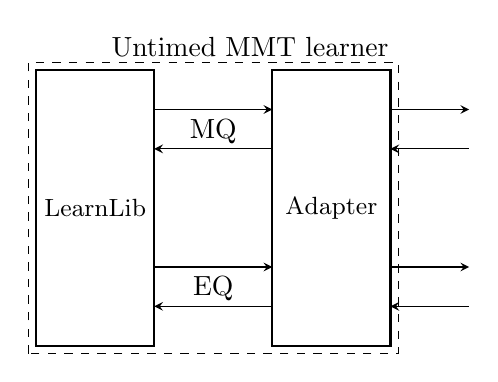
\begin{tikzpicture}[>=stealth]
 \draw [dashed] (-0.1,-0.1) rectangle (4.6,3.6);
 \node[above, left] at (4.6,3.8) {Untimed MMT learner};
            \draw [thick] (0,0) rectangle (1.5,3.5) node[midway] {\small LearnLib};
            \draw [thick] (3,0) rectangle (4.5,3.5) node[midway] {\small Adapter};
            \draw [->] (1.5,3) -- (3,3) node[midway,below] {MQ};
            \draw [<-] (1.5,2.5) -- (3,2.5);
            \draw [->] (1.5,1) -- (3,1) node[midway,below] {EQ};
            \draw [<-] (1.5,0.5) -- (3,0.5);
            \draw [->] (4.5,3) -- (5.5,3);
            \draw [<-] (4.5,2.5) -- (5.5,2.5);
            \draw [->] (4.5,1) -- (5.5,1);
            \draw [<-] (4.5,0.5) -- (5.5,0.5);
        \end{tikzpicture}
\end{center}
We assume learner knows bound $n$ on the number of timers that can be active in a state. Adapter uses function \red{$\mathit{uncan}$}\ to translate canonical behaviors to behaviors involving at most $n$ clocks.
}

\frame{
\frametitle{Building an untimed MMT teacher with a timed teacher}

\begin{center}
 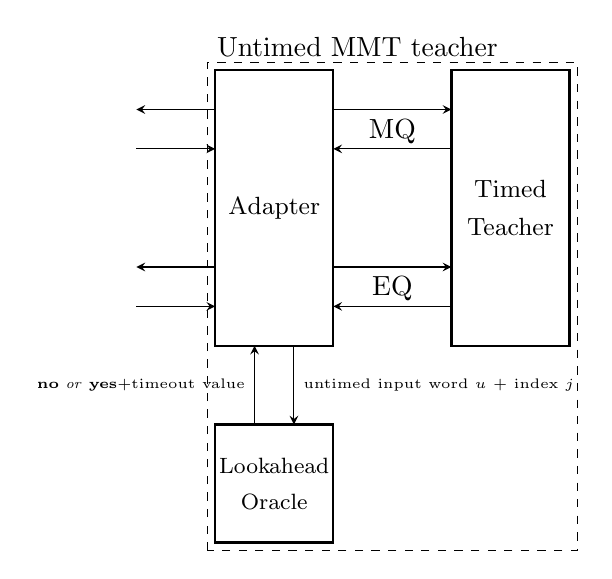
\begin{tikzpicture}[>=stealth]
 \draw [dashed] (-0.1,-2.6) rectangle (4.6,3.6);
 \node [above,right] at (-0.1,3.8) {Untimed MMT teacher};
            \draw [thick] (0,0) rectangle (1.5,3.5) node[midway] {\small Adapter};
            \draw [thick] (3,0) rectangle (4.5,3.5) node[midway,above] {\small Timed}; 
            \draw [thick] (3,0) rectangle (4.5,3.5) node[midway,below] {\small Teacher};
            \draw [->] (1.5,3) -- (3,3) node[midway,below] {MQ};
            \draw [<-] (1.5,2.5) -- (3,2.5);
            \draw [->] (1.5,1) -- (3,1) node[midway,below] {EQ};
            \draw [<-] (1.5,0.5) -- (3,0.5);
            \draw [->] (0,3) -- (-1,3);
            \draw [<-] (0,2.5) -- (-1,2.5);
            \draw [->] (0,1) -- (-1,1);
            \draw [<-] (0,0.5) -- (-1,0.5);
            \draw [thick] (0,-2.5) rectangle (1.5,-1) node[midway,below] {\footnotesize Oracle};
            \draw [thick] (0,-2.5) rectangle (1.5,-1) node[midway,above] {\footnotesize Lookahead};
            \draw [->] (0.5,-1) -- (0.5,0) node[midway,left] {\tiny {\bf no} \emph{or} {\bf yes}+timeout value};
            \draw [->] (1,0) -- (1,-1) node[midway,right] {\tiny untimed input word $u$ + index $j$};
        \end{tikzpicture}
\end{center}

}

\frame{
\frametitle{Query complexity}

Number of queries \red{polynomial}\  in size canonical MMT $\N$ produced by Myhill-Nerode construction.

\vspace{1 em}
This MMT may be \red{exponentially}\  bigger (in the number of clocks) than original MMT $\M$ of the teacher (cf register automata).

\vspace{1 em}
\blue{For MMTs with single timer, learning is easy}: all untimed behaviors are feasible, lookahead oracle is trivial if we assume learner
knows bound on maximal timer value (just wait), and complexity is the same as for Mealy machine with the same size.
}

\section{Conclusions and future work}
\frame{
\frametitle{Conclusions}
Our work consitutes a major step towards a practical approach for active learning of timed systems. 

\vspace{1 em}
Just like timed automata paved the way to extend 
model checking to a timed setting, we expect that MMTs will
make it possible to lift model learning to a timed setting.
}

\frame{
\frametitle{Future Work}
\begin{enumerate}
\item
Implement equivalence oracle
\item
Implement lookahead oracle (inspired by Tomte tool)
\item
Handle non transparent counterexamples
\item
Deal with timing uncertainty in real applications
\item
Implement our algorithm and apply to practical case studies
\item
Many theoretical questions left!
\end{enumerate}
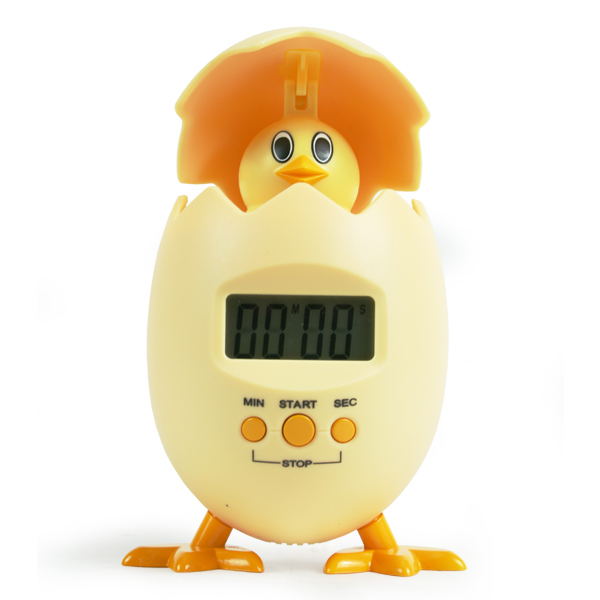
\includegraphics[width=.2\textwidth]{egg_timer0.jpg}
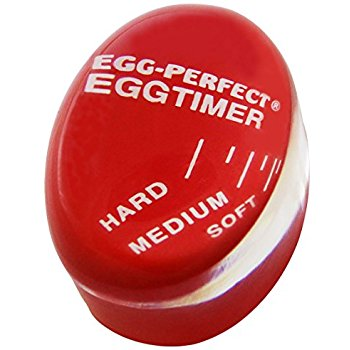
\includegraphics[width=.2\textwidth]{egg_timer2.jpg}
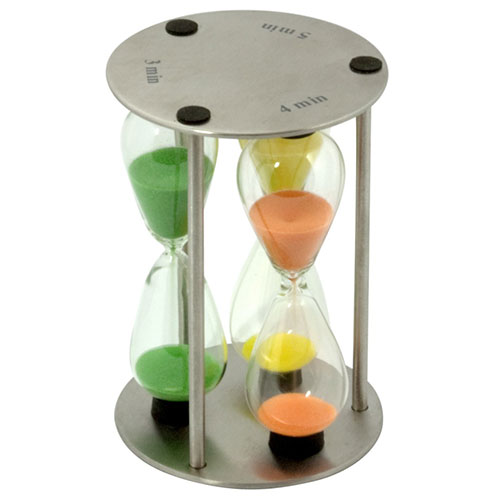
\includegraphics[width=.2\textwidth]{Sand-timer.jpg}
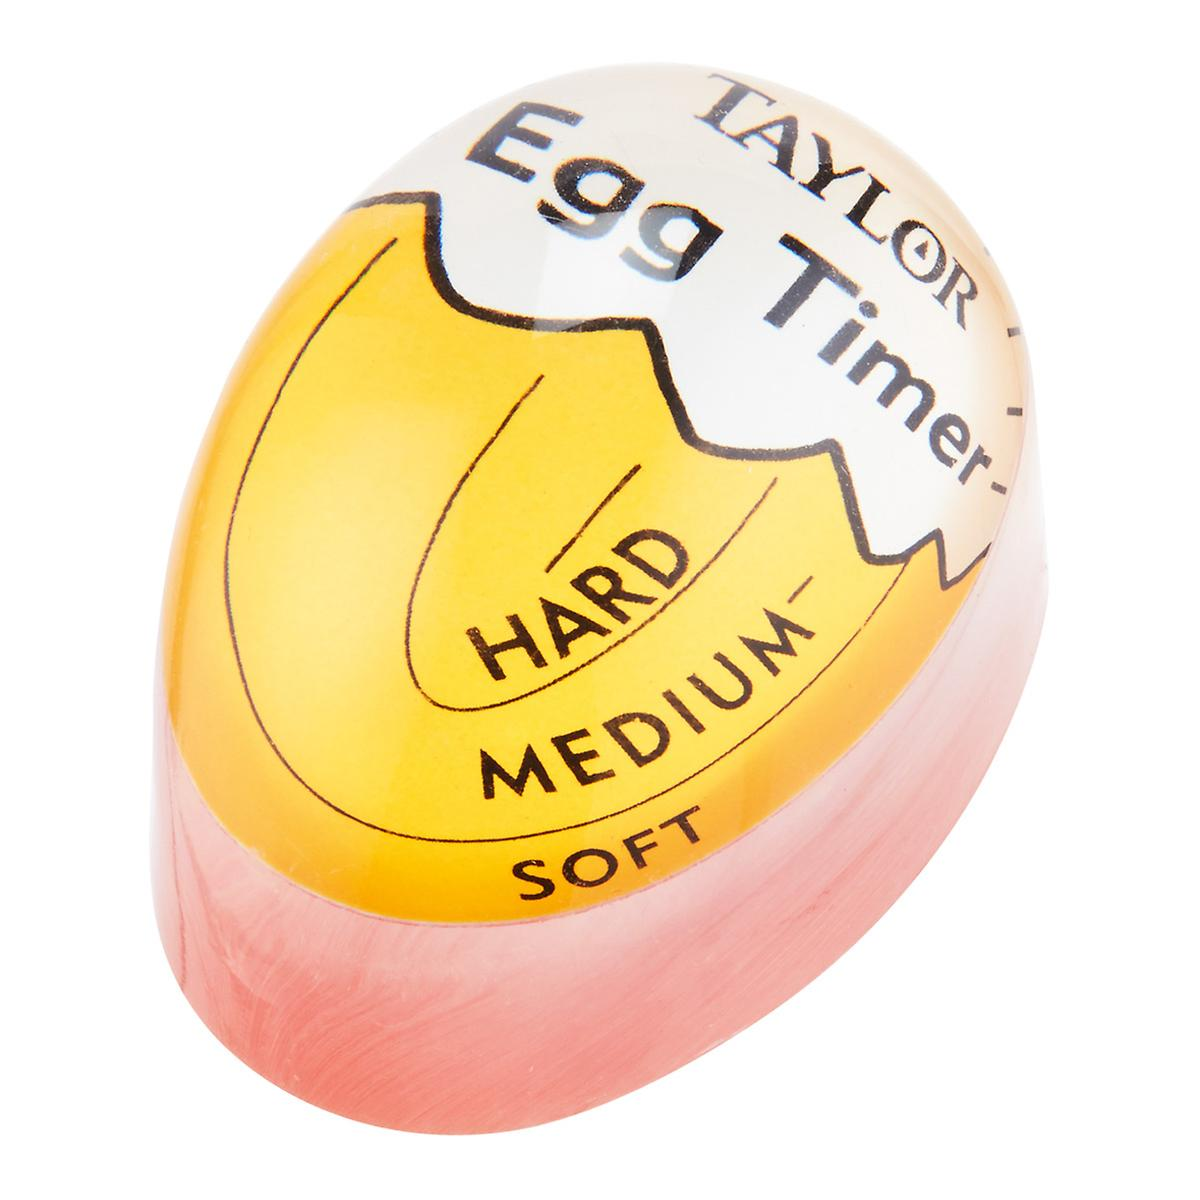
\includegraphics[width=.2\textwidth]{egg_timer3.jpg}
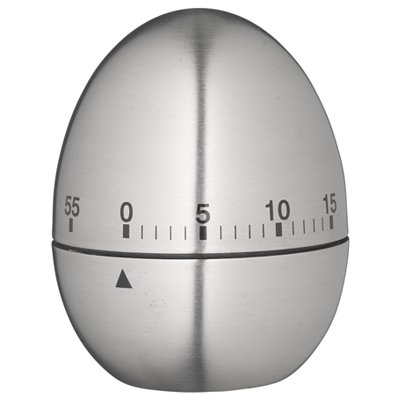
\includegraphics[width=.2\textwidth]{egg_timer4.jpg}
}





\end{document}
